\chapter{ЧИСЛЕННОЕ РЕШЕНИЕ ОСНОВОПОЛАГАЮЩИХ УРАВНЕНИЙ} \label{ch3}

\section{Численное решение уравнения движения}

Поставим задачу представить уравнение движения релятивистской частицы в удобном для численного расчёта виде. Запишем уравнение движения в общем виде
\begin{equation}
\frac{d \vec{p}}{dt} = \vec{F},
\label{eq:Newton_for_numeric}
\end{equation}
где $\vec{p}$ --- импульс частицы, а $\vec{F}$ --- сила действующая на частицу. 

Есть несколько подходов к разрешения данной задачи.

\subsection{Численное решение уравнения движения через импульс частицы}


Известны релятивистские соотношения для полной энергии $\mathscr{E}$ и для импульса:
\begin{eqnarray*}
	\mathscr{E} &=& \frac{mc^2}{\sqrt{1 - v^2/c^2}},\\ \nonumber \\
	\vec{p} &=& \frac{m\vec{v}}{\sqrt{1 - v^2/c^2}}.
\end{eqnarray*}
Отсюда следует, что
\begin{equation}
	\vec{v} = \frac{\vec{p}c^2}{\mathscr{E}}.
\end{equation}
С другой стороны, известно, что $\mathscr{E} = \sqrt{p^2c^2 + m^2 c^4}$.
Принимая во внимания определение скорости, запишем
\begin{equation}
	\frac{d\vec{r}}{dt} = \frac{c \vec{p}}{\sqrt{p^2 + m^2 c^2}}.
	\label{eq:drdt_rel}
\end{equation}
Тогда из \eqref{eq:Newton_for_numeric} и \eqref{eq:drdt_rel} несложно получить систему из шести дифференциальных уравнения первого порядка:
\begin{equation}
	\begin{cases}
	\dot{p}_x = F_x, \qquad \dot{p}_y = F_y, \qquad \dot{p}_z = F_z, \\ \\
	\dot{x} = \dfrac{c p_x}{\sqrt{p^2 + m^2 c^2}}, \\ \\
	\dot{y} = \dfrac{c p_y}{\sqrt{p^2 + m^2 c^2}}, \\ \\
	\dot{z} = \dfrac{c p_z}{\sqrt{p^2 + m^2 c^2}}.
	\end{cases}
	\label{eq:style1}
\end{equation}

\subsection{Численное решение уравнения движения через ускорение частицы}

Расписав полную производную по времени в \eqref{eq:Newton_for_numeric}, имеем
\begin{equation}
\beta \frac{d \vec{v}}{dt} + \frac{\beta^3}{c^2} (\vec{v} \cdot \frac{d \vec{v}}{dt}) \vec{v} = \vec{f},
\end{equation}
где $\vec{f} = \vec{F}/m$ --- приведённая сила. Перейдя к компонетной записи, запишем
\begin{eqnarray*}
\begin{cases}
\dot{v}_x \beta \left(1 + \frac{\beta^2}{c^2} v_x^2 \right) +
\dot{v}_y \frac{\beta^3}{c^2} v_x v_y + 
\dot{v}_z \frac{\beta^3}{c^2} v_x v_z  = f_x, \\

\dot{v}_x \frac{\beta^3}{c^2} v_x v_y +
\dot{v}_y \beta \left(1 + \frac{\beta^2}{c^2} v_y^2 \right) + 
\dot{v}_z \frac{\beta^3}{c^2} v_y v_z  = f_y, \\

\dot{v}_x  \frac{\beta^3}{c^2} v_x v_z +
\dot{v}_y \frac{\beta^3}{c^2} v_y v_z + 
\dot{v}_z \beta \left(1 + \frac{\beta^2}{c^2} v_z^2 \right)  = f_x.
\end{cases}
\end{eqnarray*}

Решим данную систему методом Крамера относительно $\dot{v}_x$, $\dot{v}_y$ и $\dot{v}_z$. 
Главный определитель:
\begin{equation*}
\Delta = \beta^3 + \beta^5 \frac{v^2}{c^2} \neq 0.
\end{equation*}
Побочные определители:
\begin{eqnarray*}
\Delta_x &=& f_x \beta^2 \left( 1+ \frac{\beta^2}{c^2} (v^2_y +  v_z^2) \right)  - f_y \frac{\beta^4}{c^2} v_x v_y - f_z \frac{\beta^4}{c^2} v_x v_z, \\ \\
\Delta_y &=& -f_x \frac{\beta^4}{c^2} v_x v_y + f_y \beta^2 \left( 1 + \frac{\beta^2}{c^2}(v_x^2 + v_z^2) \right)  - f_z \frac{\beta^4}{c^2} v_y v_z, \\ \\
\Delta_z &=& - f_x \frac{\beta^4}{c^2} v_x v_z - f_y \frac{\beta^4}{c^2} v_y v_z + f_z \beta^2 \left( 1 + \frac{\beta^2}{c^2} (v_x^2 +  v_y^2) \right).
\end{eqnarray*}
Тогда решение запишется в виде \cite{iliin_algebra}
\begin{equation*}
\dot{v}_x = \frac{\Delta_x}{\Delta}, \qquad \dot{v}_y = \frac{\Delta_y}{\Delta}, \qquad \dot{v}_z = \frac{\Delta_z}{\Delta}.
\end{equation*}
То есть
\begin{equation*}
\begin{cases}
\dot{v}_x = \dfrac{f_x (1+ \frac{\beta^2}{c^2}  [ v^2_y +  v_z^2 ]) - \frac{\beta^2}{c^2} ( f_y v_x v_y + f_z v_x v_z) }{\beta \left( 1 + \frac{\beta^2 v^2}{c^2}\right) }, \\ \\

\dot{v}_y = \dfrac{-f_x \frac{\beta^2}{c^2} v_x v_y + f_y (1 + \frac{\beta^2}{c^2} [v_x^2 + v_z^2]) - f_z \frac{\beta^2}{c^2} v_y v_z }{\beta \left( 1 + \frac{\beta^2 v^2}{c^2} \right) }, \\ \\

\dot{v}_z = \dfrac{- f_x \frac{\beta^2}{c^2} v_x v_z - f_y \frac{\beta^2}{c^2} v_y v_z + f_z (1 + \frac{\beta^2}{c^2} [v_x^2 + 2 v_y^2]) }{\beta \left( 1 + \frac{\beta^2 v^2}{c^2}\right) }. 
\end{cases}
\end{equation*}
Преобразовав, получим систему из шести дифференциальных уравнения первого порядка:

\begin{equation}
\begin{cases}
\dot{v}_x = \dfrac{f_x  + \frac{\beta^2}{c^2} \left[ f_x \left(v_y^2 + v_z^2\right) - f_y v_x v_y  - f_z v_x v_z  \right] }{\beta^3 }, \\ \\

\dot{v}_x = \dfrac{f_y  + \frac{\beta^2}{c^2} \left[ f_y \left(v_x^2 + v_z^2\right) - f_x v_x v_y  - f_z v_y v_z  \right] }{\beta^3}, \\ \\

\dot{v}_x = \dfrac{f_z  + \frac{\beta^2}{c^2} \left[ f_z \left(v_x^2 + v_y^2\right) - f_x v_x v_z  - f_y v_y v_z  \right] }{\beta^3}, \\ \\

\dot{x} = v_x, \qquad \dot{y} = v_y, \qquad \dot{z} = v_z.
\end{cases}
\label{eq:style2}
\end{equation}
Стоит напомнить, что
\begin{equation*}
\beta = \frac{1}{\sqrt{1 - v^2/c^2}} = \frac{1}{\sqrt{1 - \frac{v_x^2 + v_y^2 + v_z^2}{c^2}}}.
\end{equation*}

\subsection{Выбор метод решения системы ДУ, метод Рунге-Кутты}

В качестве метода решения системы дифференциальных уравнений (ДУ) был выбран метод Рунге-Кутты 4-го порядка. Данный метод сочетает в себе как довольно небольшое количество математических операций за один шаг, так и очень высокую сходимость\cite{butcher1987numerical}.

Суть метода заключается в следующем. Пусть имеется система ДУ:
\begin{equation*}
	\begin{cases}
		\dot{y}_1 = g_1 (t,y_1,y_2,\dots,y_n), \\
		\dot{y}_2 = g_2 (t,y_1,y_2,\dots,y_n), \\
		\vdots \\
		\dot{y}_n = g_n (t,y_1,y_2,\dots,y_n), 
	\end{cases}
	\qquad 
	\begin{cases}
		y_1 (t_0) = y_{01}, \\
		y_2 (t_0) = y_{02}, \\
		\vdots \\
		y_n (t_0) = y_{0n} 
	\end{cases}
\end{equation*}
или
\begin{equation*}
\dot{\vec{y}} = \vec{g} \left(t , \vec{y}\right), \qquad \vec{y}(0) = \vec{y}_0.
\end{equation*}
Тогда приближенное значение в последующих точках вычисляется по итерационной формуле:
\begin{equation}
\vec{y}_{n+1} = \vec{y}_n + \frac{1}{6} \left( \vec{k}_1 + 2 \vec{k}_2 + 2 \vec{k}_3 + \vec{k}_4  \right),
\end{equation}
где 
\begin{eqnarray}
\vec{k}_1 &=& \vec{g}(t_n,\vec{y}_n) dt, \nonumber \\ \nonumber \\
\vec{k}_2 &=& \vec{g}(t_n + \dfrac{dt}{2},\vec{y}_n + \dfrac{1}{2} \vec{k}_1 ) dt, \nonumber \\  \\
\vec{k}_3 &=& \vec{g}(t_n + \dfrac{dt}{2},\vec{y}_n + \dfrac{1}{2} \vec{k}_2 ) dt, \nonumber \\ \nonumber \\
\vec{k}_4 &=& \vec{g}(t_n + dt,\vec{y}_n + \vec{k}_3) dt, \nonumber
\end{eqnarray}
а $dt$ --- шаг по времени.

Этот метод имеет четвёртый порядок точности, то есть суммарная ошибка на конечном интервале интегрирования имеет порядок $\mathscr{O}(d t^4)$.



\subsection{Выбор математического ядра}

С математической точки зрения решения \eqref{eq:style1} и \eqref{eq:style2} эквивалентны относительно конечного результата. Однако задача стоит в расстановке приоритетов с точки зрения их численного решения. 

Решение \eqref{eq:style1} или т.н. <<импульсное>> решение имеет меньшее количество математических операций для расчёта. С другой стороны в нём никак явным образом не отражено ограничение на скорость частицы.

Решение \eqref{eq:style2} же более трудоёмкое с точки зрения расчётов, однако в нём явным образом исключён факт превышения скорости $c$.

Численный эксперимент показал, что при моделировании электрона в сильном однородном электрическом поле и высокой начальной скорости <<импульсное>> в конце-концов расходится при $v \lesssim c$, а именно наступает момент, когда $v>c$, что физически неверно. Решение \eqref{eq:style2} при тех же условиях ведёт себя стабильно. Однако при низких релятивистских скоростях при одном и том же шаге временной дискретизации <<импульсный>> подход даёт более высокую точность решения.


\section{Алгоритм программы для вычисления эволюции ансамбля заряженных частиц}

Основная идея вычислительной программы заключается в следующем. При каждом запуске в первую очередь идёт загрузка входных данных (параметры пространственной и временной дискретизации, информация о внешних электромагнитных полях, параметры частиц, такие как плотность и температура, и~др.). Далее происходит инициализация (задание начальных координат и скоростей) первоначальных частиц в системе. После этого уже начинается выполнение основного цикла по времени, в котором уже происходит расчёт поля пространственного заряда и решение уравнений движения для всех заряженных частиц (рисунок \ref{fig:Diagram1}). 

\begin{figure}[h!]
\centering
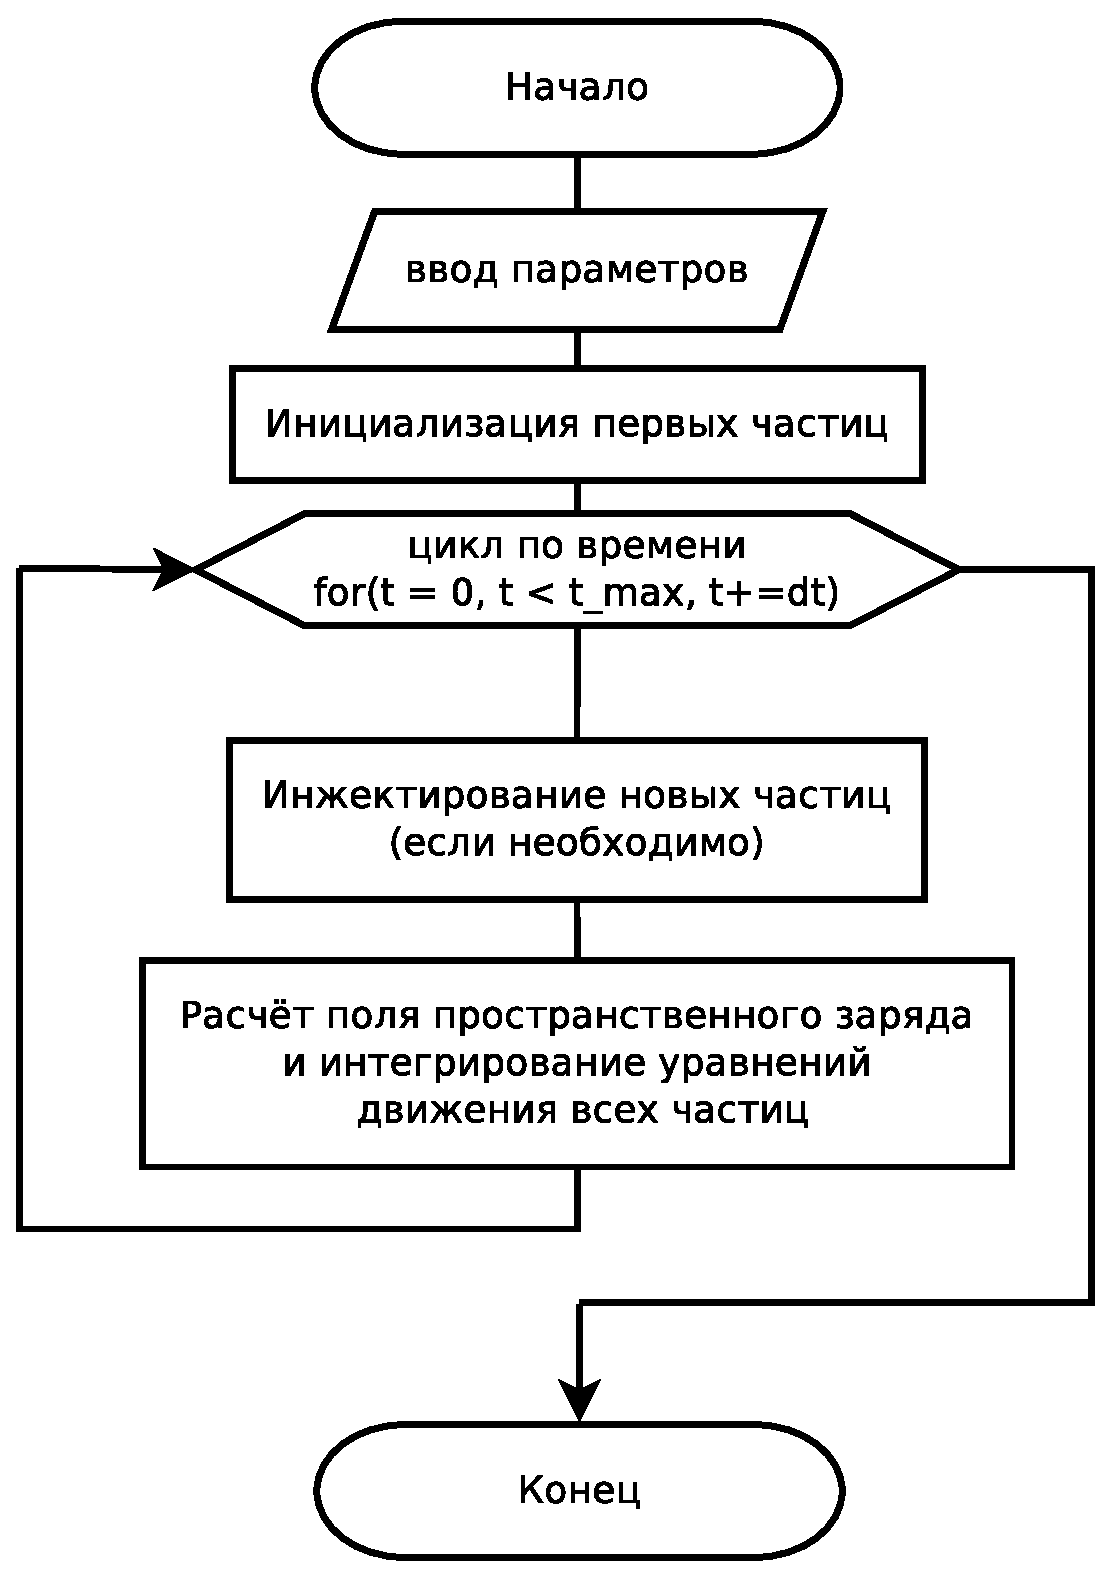
\includegraphics[width=0.5\linewidth]{./fig/ch3/Diagram1}
\caption{Упрощенный базовый алгоритм вычислительной программы}
\label{fig:Diagram1}
\end{figure}

Алгоритм вычислительной программы может значительно различаться в зависимости от того, каким образом рассчитывается поле пространственного заряда. 

В самом общем случае это выражения для полей, полученные из потенциалов Лиенара-Вихерта \cite{Landau2}:
\begin{equation}
	\vec{E} = \dfrac{q}{4 \pi \varepsilon_0} \dfrac{\left( 1 - \dfrac{v^2}{c^2} \right) \left( \vec{R} - \dfrac{\vec{v} R}{c}  \right) }{\left( R - \dfrac{\vec{v} \cdot \vec{ R}}{c} \right)^3} + \dfrac{q}{4 \pi \varepsilon_0 c^2} \dfrac{\left[ \vec{R} , \left[ \vec{R} - \dfrac{\vec{v}R}{c} , \dot{\vec{v}}  \right]  \right]}{\left( R - \dfrac{\vec{v} \cdot \vec{ R}}{c} \right)^3},
	\label{eq:opt_LV_E_early}
\end{equation}
\begin{equation}
	\vec{B} = \frac{1}{c} \frac{\vecmult{R}{E}}{R}.
	\label{eq:opt_LV_B_early}
\end{equation}
Здесь $\vec{R}$ --- радиус вектор, направленный от частицы с зарядом $q$ до точки, в которой рассчитывается поле;  $\dot{\vec{v}} = \partial \vec{v} / \partial \tau$. Все величины в правых сторонах берутся в момент времени $\tau$, определяемым уравнением 
\begin{equation}
	\tau = t - \frac{R(\tau)}{c}.
	\label{eq:wait_for_me}
\end{equation}


Выражения \eqref{eq:opt_LV_E_early} и \eqref{eq:opt_LV_B_early} были получены не используя никакие пренебрежения и упрощения (за исключением представления частицы точечной). В остальном же они учитывают все возможные эффекты, в том числе и излучение при $\dot{\vec{v}} \neq 0$. Однако, плата за такую полноту описания является огромная вычислительная сложность решения. Рассмотрим возможные упрощения и предельные переходы, которые можно сделать.

Первое возможное предположение --- это пренебрежение временем запаздывания, то есть от него ничего не должно зависеть. Отсюда следует, что $\partial \vec{v}/\partial \tau \to 0$.
тогда выражения \eqref{eq:opt_LV_E_early}, \eqref{eq:opt_LV_B_early} редуцируются в следующие:
\begin{eqnarray}
	\vec{E} &=& \dfrac{q}{4 \pi \varepsilon_0} \dfrac{\left( 1 - \dfrac{v^2}{c^2} \right) \left( \vec{R} - \dfrac{\vec{v} R}{c}  \right) }{\left( R - \dfrac{\vec{v} \cdot \vec{ R}}{c} \right)^3} , \\ \nonumber \\
	\label{eq:opt_LV_E_easy}
	\vec{B} &=& \dfrac{1}{c} \frac{\vecmult{R}{E}}{R}.
	\label{eq:opt_LV_B_easy}
\end{eqnarray}

Следующим шагом в упрощении может стать дорелятивизм. Иначе говоря, если
$v/c \to 0$,
то выражения для полей примут наиболее простой вид
\begin{eqnarray}
\vec{E} &=& \dfrac{q}{4 \pi \varepsilon_0}  \dfrac{ \vec{R} }{R^3}, \label{eq:opt_LV_E_easiest} \\ \nonumber \\
\vec{B} &=& 0.
\label{eq:opt_LV_B_easiest}
\end{eqnarray}


Рассмотрим два предельных случая --- согласно уравнениям \eqref{eq:opt_LV_E_early} и \eqref{eq:opt_LV_B_early}, которые учитывают времена запаздывания, и согласно уравнениям \eqref{eq:opt_LV_E_easiest} и \eqref{eq:opt_LV_B_easiest}.

\subsection{Релятивистское движение с учётом запаздывание}

Рассмотрим численный алгоритм расчёта полей согласно уравнениям, полученным из потенциалов Лиенара-Вихерта. Основная сложность заключается в решении уравнения \eqref{eq:wait_for_me} для определения времени запаздывания $\tau$.

\begin{figure}[h!]
\centering
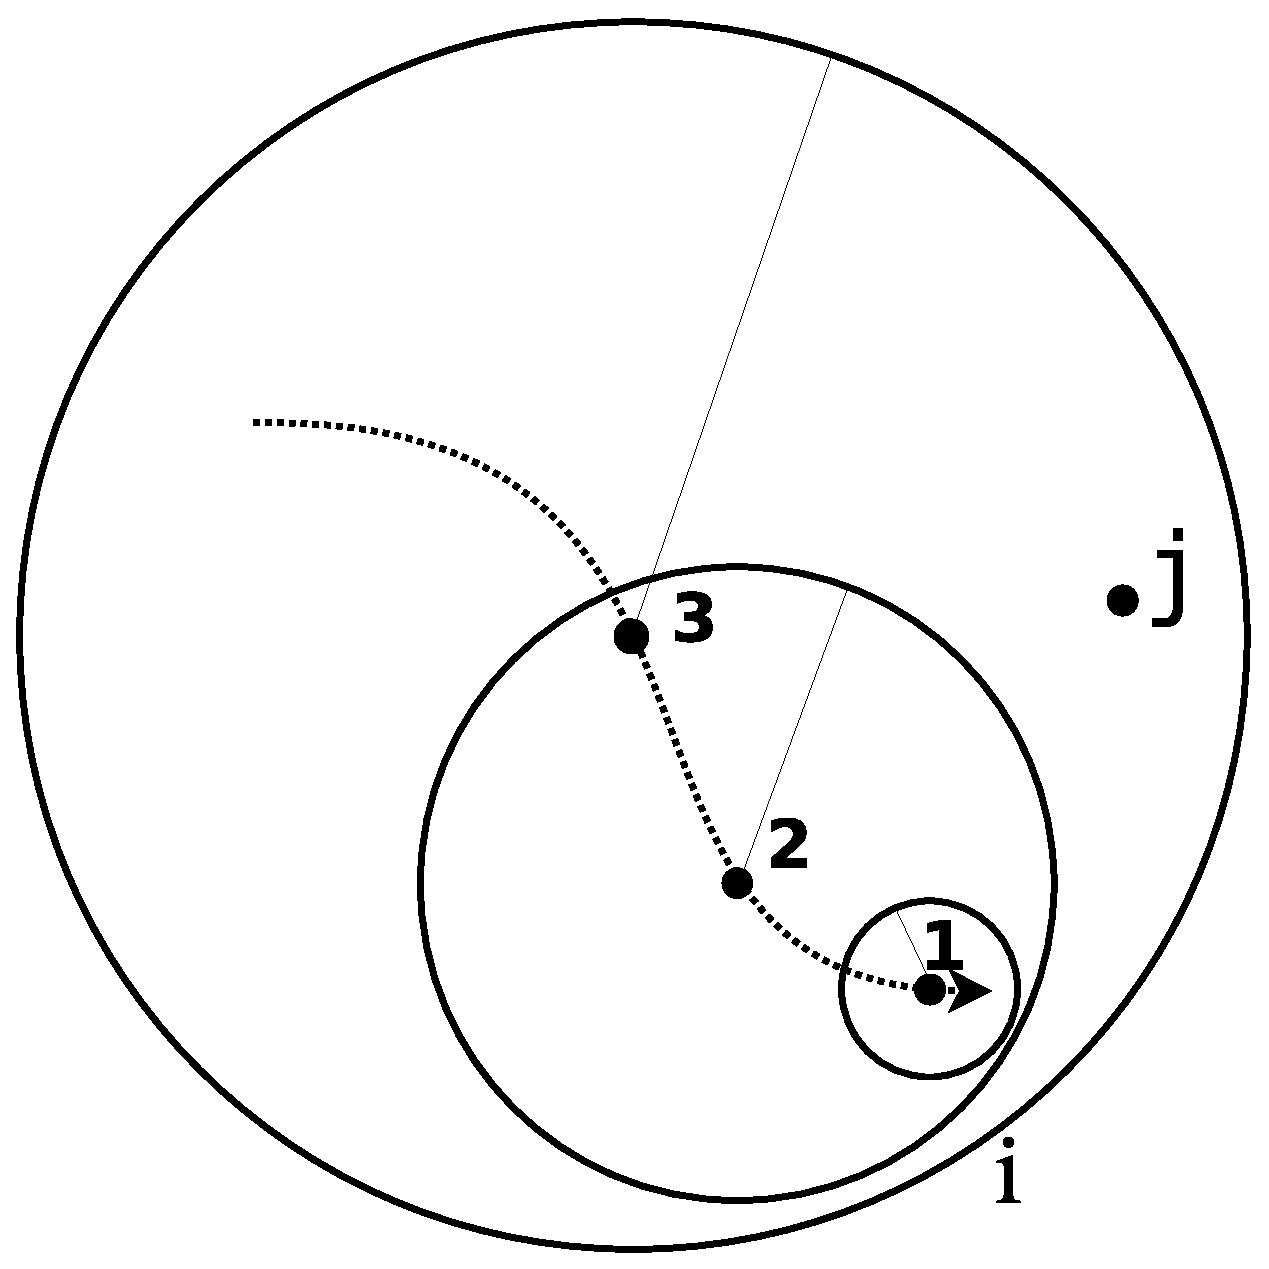
\includegraphics[width=0.5\linewidth]{./fig/ch3/Diagram2tau}
\caption{Графическое представление решения уравнения \eqref{eq:wait_for_me}}
\label{fig:Diagram2tau}
\end{figure}

Решить его можно следующим образом. Пусть есть траектория $i$-й частицы и необходимо найти то время, за которое сигнал от этой самой $i$-й частицы дошел до некоторой $j$-й частицы. Сигнал распространяется в вакууме, как известно, со скоростью $c$, значит необходимо построить сферу взаимодействия для каждого шага, радиус которой будет равен $k \cdot cdt$, $k$ --- количество шагов <<в прошлое>> (рисунок \ref{fig:Diagram2tau}). Строить данные сферы необходимо до тех пор, пока расстояние до $j$-й частицы не станет меньше радиуса сферы
\begin{equation}
r_{ij} \leqslant k' c dt,
\end{equation}
тогда
\begin{equation}
\tau = k' dt.
\end{equation}
Далее, алгоритм действий внутри цикла по времени представлен на рисунке \ref{fig:Diagram3}.

\begin{figure}[h!]
\centering
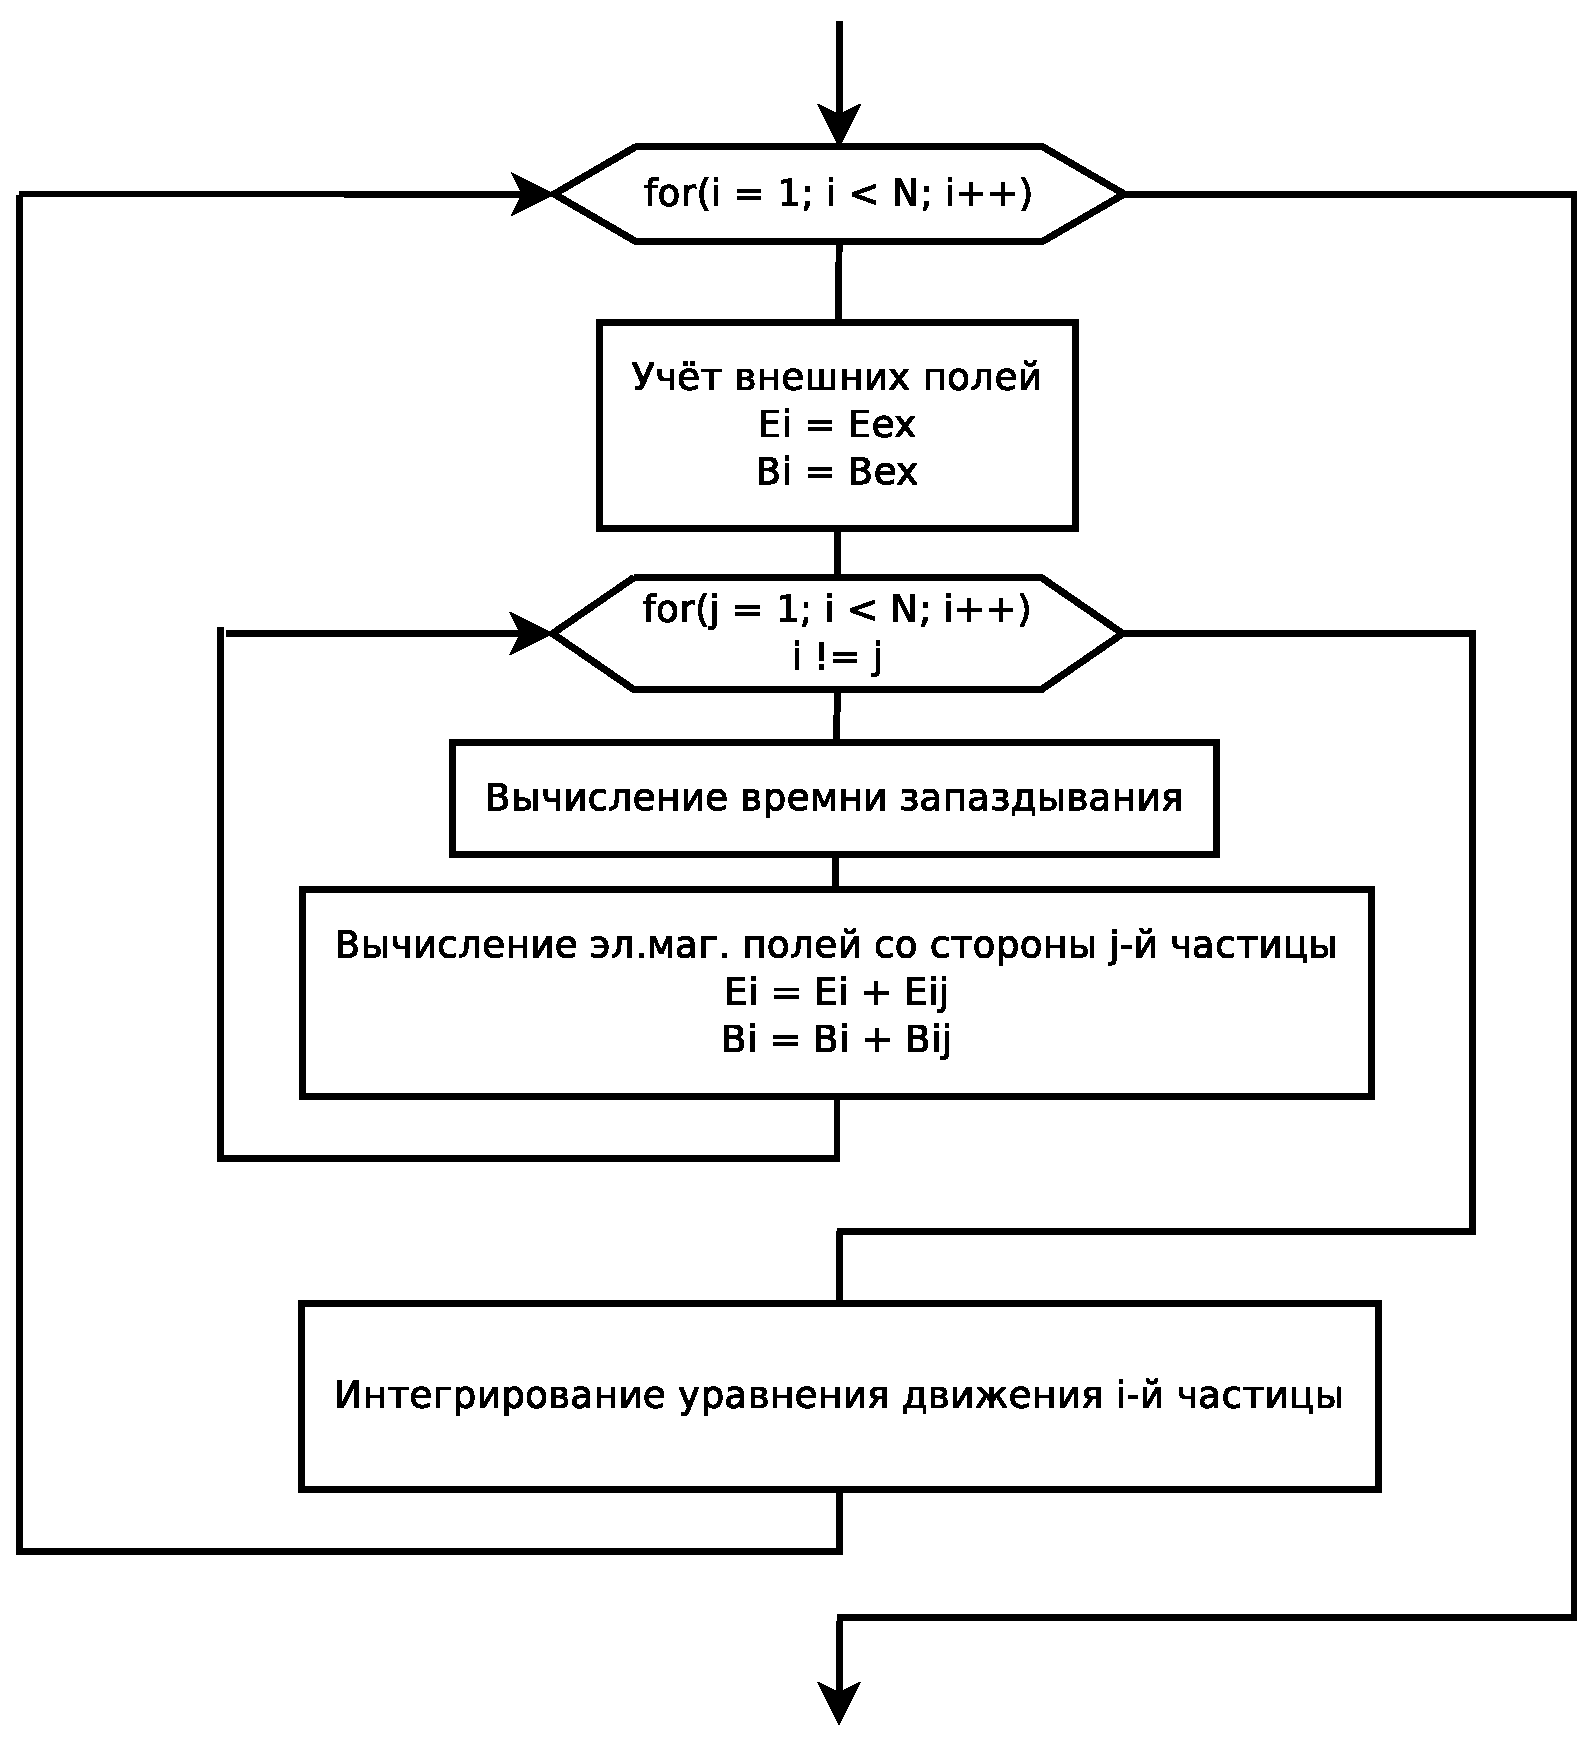
\includegraphics[width=0.7\linewidth]{./fig/ch3/Diagram3}
\caption{Алгоритм действий внутри цикла по времени с учётом потенциалов запаздывания}
\label{fig:Diagram3}
\end{figure}


\subsection{Нерелятивистское движение без учёта запаздывания}

В другом предельном случае, когда $R/c$ пренебрежительно мало и $v/c \to 0$, можно значительно ускорить процесс вычислений, если воспользоваться напрямую третьим законом Ньютона:
\begin{equation}
\vec{F}_{ij} = - \vec{F}_{ji},
\end{equation}
где $\vec{F}_{ij}$ --- сила взаимодействия $i$-й частицы на $j$-ю частицу, а $\vec{F}_{ji}$ --- наоборот.  В случае кулоновского потенциала при дебаевской экранировке сила взаимодействия будет вычисляться следующим образом:
\begin{equation*}
	\vec{F}_{ij} = - \nabla \left[U_{ij} (r_{ij}) \cdot \Phi \left( \frac{r_{ij}}{r_D} \right)\right] = - \nabla \left[ \frac{1}{4 \pi \varepsilon_0} \frac{q_i q_j}{r_{ij}} \cdot e^{r_{ij}/r_D} \right],
\end{equation*}
\begin{equation}
	\vec{F}_{ij} = 
	\begin{cases}
		\dfrac{1}{4 \pi \varepsilon_0} \dfrac{q_iq_j \left( \vec{r}_i - \vec{r}_j \right)}{r_{ij}^2} e^{-r_{ij}/r_D} \left( \dfrac{1}{r_{ij}} - \dfrac{1}{r_D} \right), & r_{ij} < r_D, \\
		0, & r_{ij} \geq r_D.
	\end{cases}
	\label{eq:force_with_debai}
\end{equation}
Простейшая оценка радиуса Дебая даёт следующее выражение
\begin{equation}
	r_D = \sqrt{\frac{\varepsilon_0 T}{q^2n}}.
	\label{eq:debai_analitic}
\end{equation}

В теле цикла по времени необходимо будет реализовать следующее:
\begin{enumerate}
\item Вычисление матриц сил
\begin{equation}
F^x_{ij}, \quad F^y_{ij}, \quad F^z_{ij},
\end{equation}
учитывая их антисимметричность $F^{\alpha}_{ij} = - F^{\alpha}_{ji}$, где $\alpha = x,y,z$.
\item Интегрирование уравнений движений, в которых сила взаимодействия на $i$-ю частицу будет определяться, как
\begin{equation}
F^{\alpha}_i = F^{\alpha}_{ex} + \sum\limits_{j} F^{\alpha}_{ij},
\end{equation}
где $F^{\alpha}_{ex}$ --- внешняя сила.
\end{enumerate}



\section{Численное решение уравнений магнитостатики}

В случае решения задач с помощью метода <<частица-частица>>, представляется затруднительным решать самосогласованные полевые задачи. Однако, режимов работы установок по удержанию плазмы, связанных с самосогласованностью электромагнитных полей не так уж и много. К ним относятся, например, эксперименты с компактным тором. В англоязычной литературе известно название Field Reversed Configuration (FRC) --- конфигурация с обращенным полем. Теория пока мало изучена, а постановка экспериментов крайне сложна \cite{Steinhauer2006, Ryzhkov2015d, Intrator2004}. Стоить отметить, что эксперименты по FRC проводятся именно на базах открытых ловушек.

\subsection{Общие положения}

Во многих задачах, особенно когда требуется получить оценочный результат, достаточно использовать уравнения магнитостатики. В случае $\partial \vec{E}/\partial t = 0$ пара уравнений максвелла становится закрытой системой:
\begin{numcases}{}
	\Div \vec{B} = 0, \\
	\Rot \vec{B} = \mu_0 \vec{j}. \label{eq:max_without_E}
\end{numcases}

А так как поле $\vec{B}$ можно представить через векторный потенциал как  $\vec{B} = \Rot \vec{A}$, то тогда, принимая во внимание формулу векторного анализа для двойного ротора, перепишем выражение \eqref{eq:max_without_E} в следующем виде
\begin{equation}
	\Grad \Div \vec{A} - \Delta \vec{A} = \mu_0 \vec{j}.
\end{equation}
Используя кулоновскую калибровку для векторного потенциала $\Div \vec{A} = 0$, получим
\begin{equation}
	\Delta \vec{A} = - \mu_0 \vec{j}. \label{eq:toSolveToFindB}
\end{equation}
Решение уравнения \eqref{eq:toSolveToFindB} можно записать в виде \cite{Landau2}
\begin{equation}
	\vec{A} = \frac{\mu_0}{4 \pi} \int \frac{\vec{j}}{R} dV,
\end{equation}
где $R$ --- радиус вектор, направленный их $dV$ в точку наблюдения. Найдя $\Rot \vec{A}$, получим так называемый закон Био--Савара
\begin{equation}
	\vec{B} = \frac{\mu_0}{4 \pi} \int \frac{\vecmult{j}{R}}{R^3} dV.
	\label{eq:bio_savar}
\end{equation}

\subsection{Случай тонкого кольца с током}

Учитывая относительные размеры и расположения магнитных катушек и камеры, где непосредственно находится плазма, можно сделать предположение, что магнитная катушка представляет собой тонкий контур с током в форме окружности радиуса $R'$. В этом случае задача значительно упрощается. 

Пусть имеется контур с током $\gamma = 2 \pi R'$, по которому течёт ток $I$. Учитывая связь $\vec{j} dV = I \vec{dl}$, перепишем выражение \eqref{eq:bio_savar} для витка с током
\begin{equation}
	\vec{B} = \frac{\mu_0}{4 \pi} \oint \limits_{\gamma = 2 \pi R'} \frac{I \cdot \vecmult{dl}{R}}{R^3}.
	\label{eq:bio_savar_curl}
\end{equation}

Перейдём в цилиндрическую систему координат $(r,\varphi,z)$. Ось $z$ направим перпендикулярно плоскости контура $\gamma$. Ток $I$, очевидно, можно вынести из под знака интеграла. Найдём модуль магнитной индукции, принимая во внимание тот факт, что у элемента $\vec{dl}$ есть только $\varphi$-я компонента:
\begin{equation}
	B = \frac{\mu_0 i}{4 \pi}  \int \limits_0^{2 \pi} \frac{R' d \varphi}{R^2} = \frac{\mu_0 R'}{2} \cdot \frac{I}{R^2}.
	\label{eq:calcBcyl}
\end{equation}
Направление вектора $\vec{B}$ будет определятся согласно правилу правого винта.
